\chapter{Background}

% To have a better understanding of our approach, it's important to understand the basic concept and assumption that we used to develop the approach. 

\section{\ac{VHR} Aerial Imagery}

\begin{figure}[H]
    \centering
    \includegraphics[width=\textwidth]{Figures/arz_7_res_compare.png}
    \caption[Resolution Comparison]{Comparison between different resolutions. From left to right, where (a) has half meter scales, (b) has 5 meter scales and (c) has 10 meter scales. With the increase of meter scale, it harder to capture the boundary of the edges detail of sidewalks.}
    \label{fig:vhr_compare}
\end{figure}
% \todo{change dpi to 5 meter scale. make it worse.}

\ac{VHR} stands for Very High Resolution. It has advantageous for buildings extraction, road detection or image segmentation~\cite{FREIRE20141, 10.1007/BFb0015525, 10.1007/978-3-642-15567-3_16}. 
These aerial imageries contain more information and detail due to the higher resolution, which gives us the ability to develop more complex analysis on the imagery with same size.
\figref{fig:vhr_compare} demonstrates the difference between different resolution within the same area. From (a) to (c), the resolution changes from half meter scale to 10 meter scale. 
With higher resolution, it is easier to find the precious boundaries of an object or identify it. 
For building extraction, higher resolution provides more information when dealing with complex houses or extract complex suburban roofs~\cite{10.1007/BFb0015525}. 
For thin ribbon-features segmentation such as sidewalks in our approach, to visualize an overlaid map without high resolution, the imagery can be distracting, and the output may be effected by tiny discrepancies between digitized pathways~\cite{10.1007/978-3-642-15567-3_16}. 

\section{\ac{OSM}}
\begin{figure}[H]
    \centering
    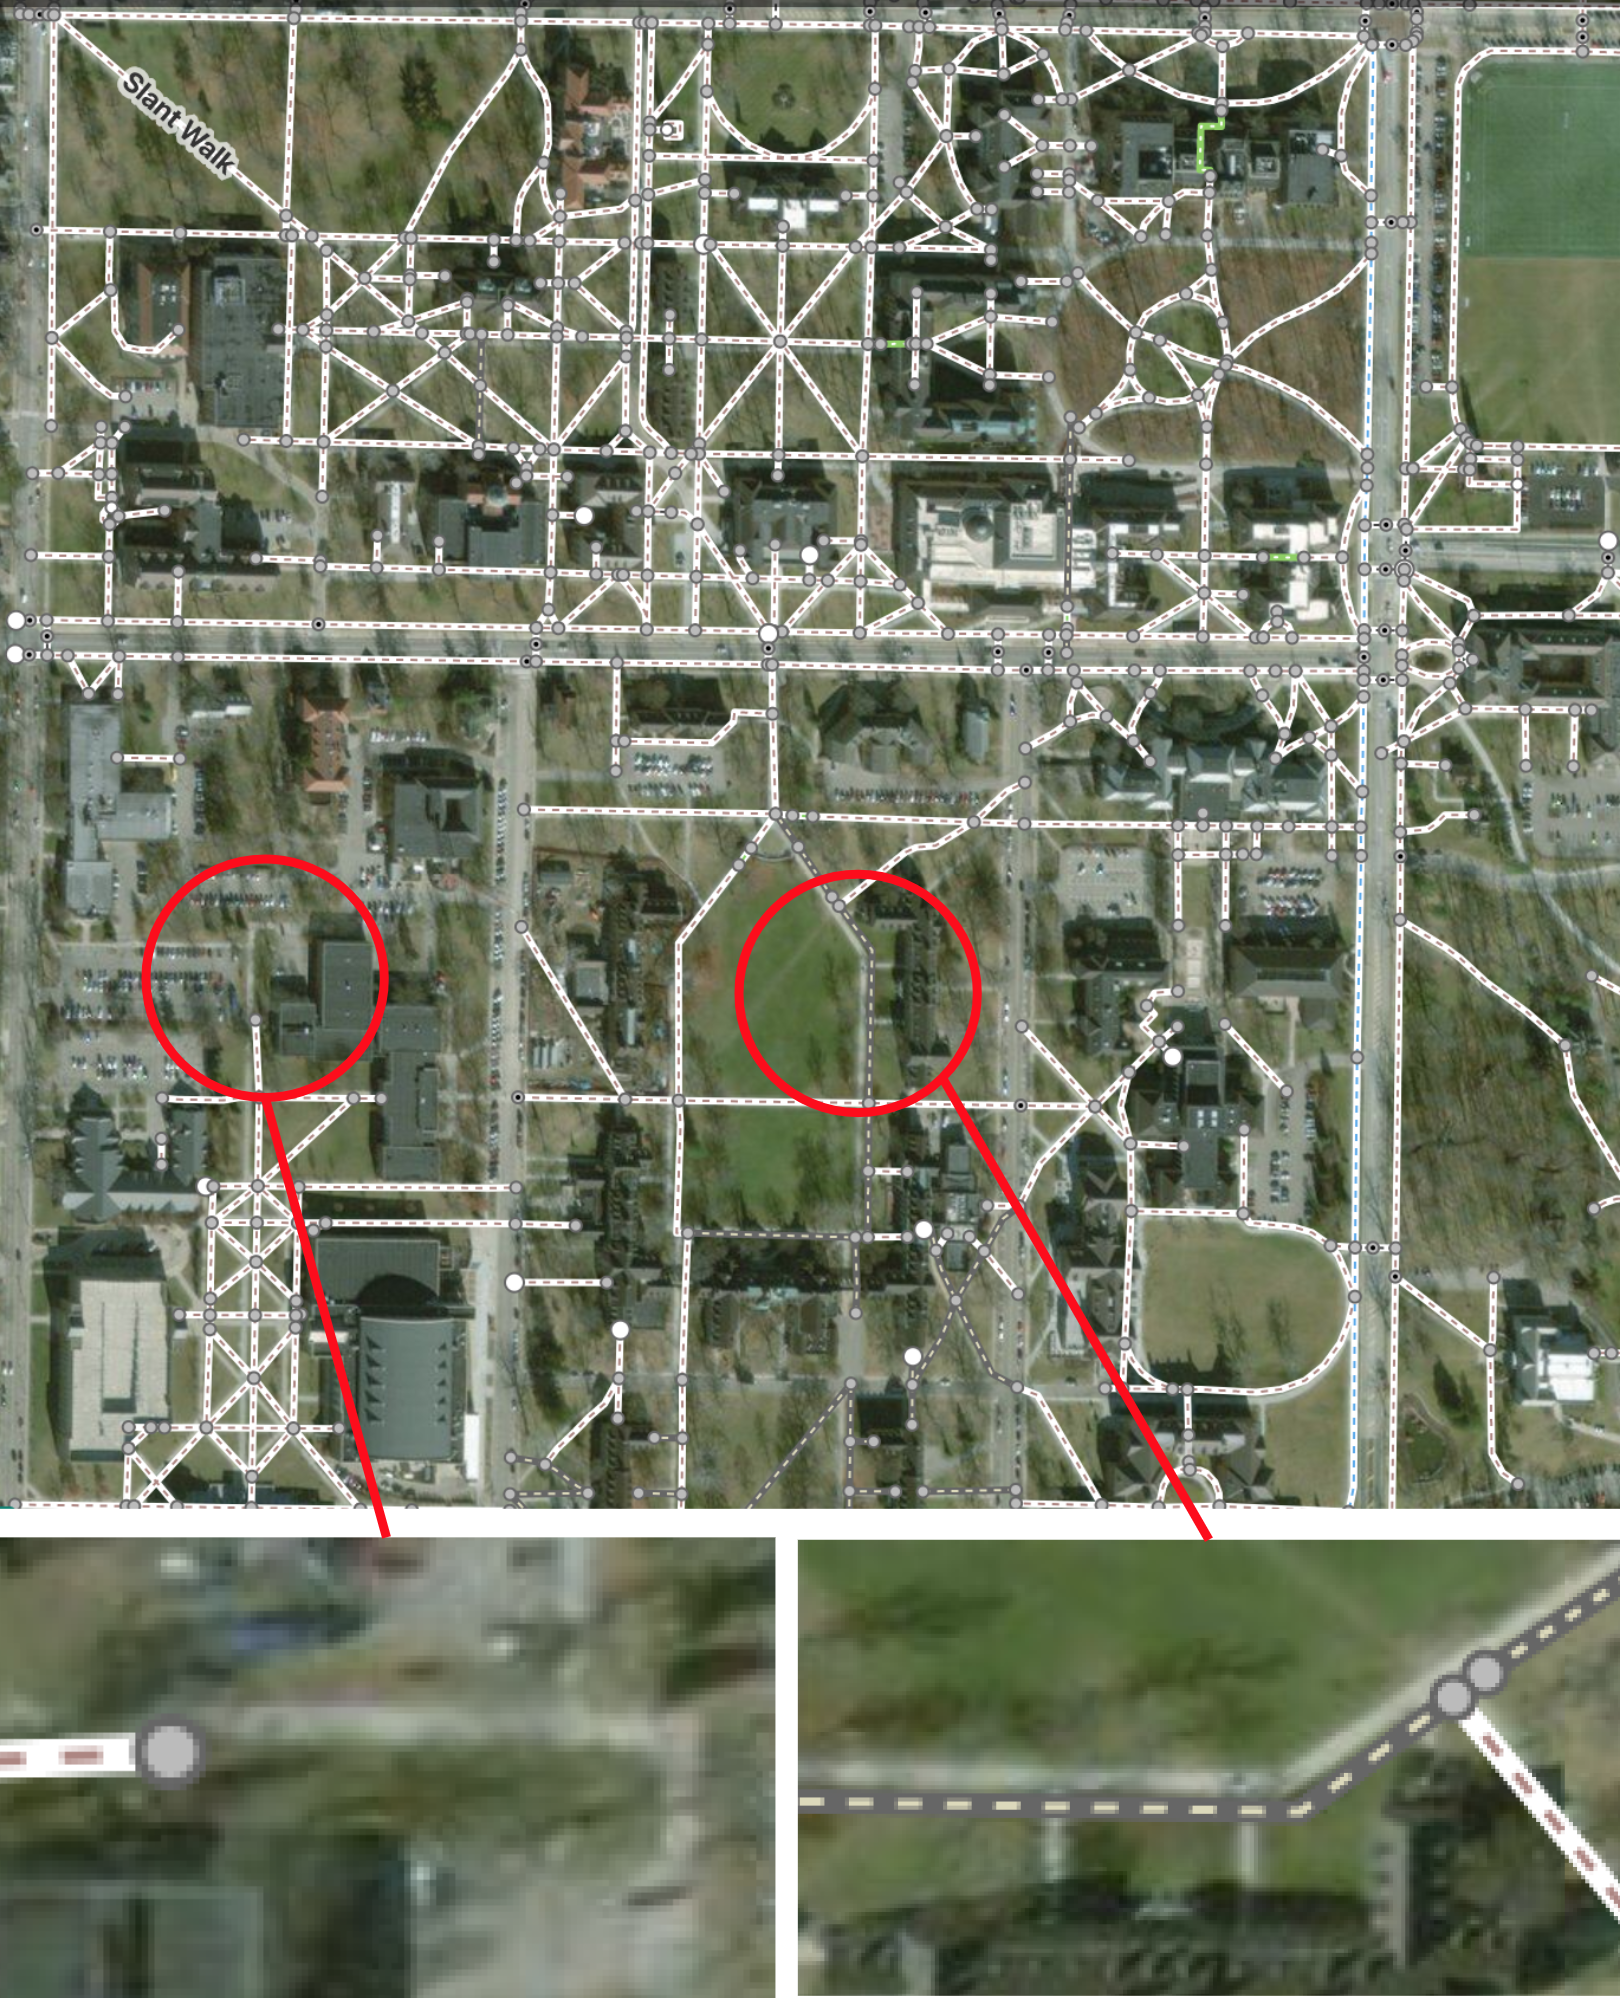
\includegraphics[width=0.85\textwidth]{Figures/oxford_path_data_osm.png}
    \caption[\ac{OSM} Walking Path]{A demonstration of actual walking path data from \ac{OSM}. The figure shows in the Oxford area in Ohio, US. Row 2 specifies the zoom in version of error that we need to facing. The sidewalk misses in the path data (left), the path data marks offset compare to the actual sidewalk(right).}
    \cite{OpenStreetMap}
    \label{fig:osm_oxford_path}
\end{figure}

\ac{OSM} stands for Open Street Map, which was founded by Steve Coast in 2004~\cite{lasPiñas, OpenStreetMap}. 
\ac{OSM} is a collaborative project that allows users to generate a free editable map of the world~\cite{4653466}.
Rather than the map itself, \ac{OSM} generates the data with the map information that across most of the world as primary output. 
It also allows users to develop the map data with portable satellite navigation devices. 
With all these convenience features, \ac{OSM} is helpful for the map analysis and features segmentation~\cite{10.1007/11744078_9}. 
\figref{fig:osm_oxford_path} shows that \ac{OSM} supports features like footpaths, roads, buildings, and others, with the ability to extract the \ac{GIS} data for any individual feature. 
It may also leads to the issue of dealing with missing or invalid data when we rely on the data set for auto-detection, or mismatch data with imagery when structures changes along with time.

\section{\ac{CRF}}
\ac{CRF} stands for Conditional Random Field, which is a class of statistical modeling methods that often applied in pattern recognition and machine learning~\cite{MAL-013}. 
As a type of discriminative undirected probabilistic graphical model, \ac{CRF} is commonly used for segmenting, labeling or parsing of sequential data, such as in computer vision, structure segmentation and object recognition~\cite{RuizSarmiento2015UPGMppA, 1315232, lafferty2001conditional}. 
For road segmentation, several approaches are able to locate the precise boundaries by treating it as a \ac{CRF} problem~\cite{ActiveContou09, Achanta:149300}. 

\section{\ac{GMM}}

\ac{GMM} stands for Gaussian Mixture Models~\cite{sridharan2014gaussian}.
It is a probabilistic model for representing normally distributed subpopulations within an overall population.
\ac{GMM} often can be performed when the data points are mixtures of a Gaussian distribution. 
It can be used in common computer vision tasks such as background and foreground subtraction~\cite{1333992}. 
For road segmentation, we can treat the problem as subtract foreground (road feature) from the complex background (non-road feature). 
\figref{fig:gmm_sample_1} demonstrates the comparison between foreground and background \ac{GMM} on sample walking path show in gray-scale. 
For foreground subtraction, which we show in row 1 and row 3, we treat sidewalk texture as foreground and apply the \ac{GMM} algorithm to subtract it from the background (non-sidewalk texture). 
Background subtraction are shown in row 2 and row 4, we did the opposite and treat non-sidewalk part as foreground. 

\begin{figure}[H]
    \centering
    \includegraphics[width=0.85\textwidth]{Figures/GMM_needed.png}
    \caption[Density Background Subtraction]{A demonstration of apply \ac{GMM} algorithm on sample inputs, show with gray scale. From top to bottom, row 1 shows foreground density on sample path, row 2 show background density on the same sample path as row 1. Same with row 3 and 4, with different sample path. For foreground density, lighter color represent more likely to be sidewalk and darker color represent more likely to be non-sidewalk. Background density shows as the opposite.}
    \label{fig:gmm_sample_1}
\end{figure}


\section{\ac{DP}}
\begin{figure}
    \centering
    \includegraphics[width=0.9\textwidth]{Figures/longest_common_sequence.png}
    \caption[Demonstration on Longest Common Sequence]{Dynamic Programming demonstration with longest common sequence. Similar to our approach, to find the longest common sequence, it first needs to fill the table with \ac{DP} and then backtrack to find the longest path. It used in intersection detection with GPS trace~\cite{Xie2017DetectingRI}.
    }
    \label{fig:lcs_dp}
\end{figure}

\ac{DP} stands for Dynamic Programming. It is both a mathematical optimization method and a computer programming method \cite{bertsekas2005dynamic}. 
In 1950s \ac{DP} was invented by Richard Bellman\cite{bellman2013dynamic}. 
The main concept of \ac{DP} is to simplify a complicated problem by breaking it down into simpler sub-problems in a recursive manner \cite{howard1966dynamic}. 
In computer science, if a problem can break into serial sub-problems and each sub-problem can be recursively solved by finding its optimal solution, then we know that \ac{DP} are applicable. 

\figref{fig:lcs_dp} gives a example of a famous dynamic programming problem, Longest Common Sequence. To achieve the result of finding the longest common sequence, it first needs to fill the table with \ac{DP} and then backtrack to find the longest path. One method gives approach with using longest common sequence for intersection detection from GPS traces~\cite{Xie2017DetectingRI}.

Dynamic Programming has a variety of applications since it can significantly reduce the run-time \cite{bertsekas1995neuro}. 
We use Fibonacci Sequence to demonstrate the \ac{DP} process\cite{horadam1961generalized}. 
Figure \ref{fig:fbs}, row 1 shows that to calculate the $n^{th}$ Fibonacci number, it require a certain exponential rate of calculation to finish the process.
The time complexity can be reduced since it is re-calculating the previous Fibonacci number repeatedly. 
By applying \ac{DP} algorithm, we can save the previous calculated Fibonacci number and reused it when needed.
Figure \ref{fig:fbs}, row 2 indicate the same process after applying dynamic programming, we marked unnecessary steps in red X. 
By trade in linear space to save previous calculation, we can reduce the wrong time from exponential to linear.

\begin{figure}[H]
    \centering
    \includegraphics[width=\textwidth]{Figures/treewithdp.png}
    \caption[Demonstration on Fibonacci Sequence]{Representing the calculation of Fibonacci Sequence ($7^{th}$) with binary tree. Row 1 shows without applying dynamic programming, it need's certain exponential rate to calculate $n^{th}$ Fibonacci number. With the increase of $n$, the number of calculation increase significantly. Row 2 shows with dynamic programming, after saving previous calculation, it's only require linear time steps to calculate $n^{th}$ Fibonacci number. We marked unnecessary steps in red X to show it's can be skipped. }
    \cite{stack_overflow}
    \label{fig:fbs}
\end{figure}

% \begin{figure}
%     \centering
%     \includegraphics[width=\textwidth]{Figures/QVSdv_DP.png}
%     \caption[Demonstration on Fibonacci Sequence with \ac{DP}]{Representing the calculation of Fibonacci Sequence ($7^{th}$) with binary tree. With dynamic programming, after saving previous calculation, it's only require linear time steps to calculate $n^{th}$ Fibonacci number. We marked unnecessary steps in red X to show it's can be skipped.
%     }
%     % \cite{stack_overflow}
%     \label{fig:fbs_dp}
% \end{figure}

% \section{Street Network Extraction}
% boss paper, 2018 cvpr, they don't gurant to find the center of road.

